\documentclass{article}
\usepackage{float}
\usepackage[polish]{babel}
\usepackage[utf8]{inputenc}
\usepackage{polski}
\usepackage{listings} %code environment
\frenchspacing
\setcounter{tocdepth}{2}
\usepackage{graphicx}
\graphicspath{ {images/} }
\usepackage{color}

\lstdefinestyle{main}{
	keywords={
		after, always, causes, if, impossible, initially, observable, 
		partakes, releases, typically
    },
    keywordstyle={\bfseries},
    keywordstyle=[2]\textsc,
    frame=single,
}

\begin{document}
	
\begin{titlepage}

\newcommand{\HRule}{\rule{\linewidth}{0.5mm}}
\newcommand{\Action}[1]{\textsc{#1}}

\center

%----------------------------------------------------------------------------------------

\textsc{\LARGE Politechnika Warszawska}\\[0.3cm]
\textsc{\Large Wydział Matematyki i Nauk Informacyjnych}\\[0.6cm]

% logo

\includegraphics[width=2cm, height=2cm]{logo}\\[0.6cm]


\textsc{\Huge Reprezentacja wiedzy}\\[0.3cm]

%----------------------------------------------------------------------------------------

\HRule \\[0.4cm]
{ \LARGE \bfseries Raport z testów projektu grupy nr 4}\\[0.1cm]
 
%----------------------------------------------------------------------------------------

\HRule \\[0.4cm]
{  \bfseries Programy działań z akcjami współbieżnymi}\\[1.2cm]

% authors
\begin{flushright}
\Large \emph{Autorzy:}\\[0.5cm]
Dragan Łukasz\\
Flis Mateusz\\
Izert Piotr\\
Pielat Mateusz\\
Rząd Przemysław\\
Siry Roman\\
\textbf{Waszkiewicz Piotr}\\
Zawadzka Anna\\[0.9cm]

\end{flushright}

% date
\vfill
{\large \today}\\[1cm]
	


\end{titlepage}
	
\newpage

\section{Opis projektu}
Tematem testowanego przez nas projektu są programy działań z akcjami współbieznymi. Rozpatrywana klasa systemów dynamicznych spełnia następujące warunki:
\begin{itemize}
    \item Prawo inercji
    \item Niedeterminizm
    \item W języku kwerend występują akcje złożone (zbiory co najwyzej k akcji atomowych), w języku akcji jedynie akcje atomowe
    \item Pełna informacja o wszystkich akcjach atomowych i wszystkich ich skutkach bezpośrednich
    \item Z każdą akcją atomową zwiazany jest jej warunek wstepny (ew. TRUE) i końcowy (efekt akcji)
    \item Wykonywane są jedynie akcje bezkonfliktowe (żadne dwie akcje składowe nie mogą mieć wspólnych zmiennych, na które w jakimkolwiek stanie mają wpływ)
    \item Wynikiem akcji złożonej jest suma skutków wszystkich składowych akcji bezkonfliktowych
    \item Akcje mogą być niewykonalne w pewnych stanach; jeśli akcja jest niewykonalna, to każda akcja ją zawierająca jest niewykonalna
    \item Dopuszczalny jest opis częściowy zarówno stanu poczatkowego, jak i pewnych stanów wynikajacych z wykonań sekwencji akcji
\end{itemize}

Opracowywany jezyk kwerend ma za zadanie umożliwiać tworzenie zapytań,
pozwalających na uzyskanie odpowiedzi na następujace pytania:
\begin{itemize}
    \item Czy podany program P działań jest możliwy do realizacji  zawsze/kiedykolwiek ze stanu początkowego?
    \item Czy wykonanie programu P działań w stanie początkowym prowadzi zawsze/kiedykolwiek do osiągniecia celu $\gamma$?
    \item Czy cel $\gamma$ jest osiagalny ze stanu początkowego?
\end{itemize}
\newpage

\section{Przeprowadzone testy}
\subsection{Test 1}
Zdefiniowana dziedzina:
\bigskip
\lstset{
	style=main,
	keywords=[2]{Load, Shoot},
}
\begin{lstlisting}[mathescape=true]
initially alive
initially $\neg$loaded
Load causes loaded
Shoot causes $\neg$loaded if loaded
Shoot causes $\neg$alive if loaded
\end{lstlisting}
\vspace{1cm}
Zadane kwerendy:
\begin{itemize}
    \item {\large\texttt{ever accessible $\neg$alive}}\\
    Odpowiedź: \texttt{TRUE}\\
    Jest to odpowiedź poprawna, ponieważ istnieje ciąg akcji, który prowadzi do stanu spełniającego podany cel, co ilustruje poniższy graf:
    \begin{figure}[H]
    \centering
    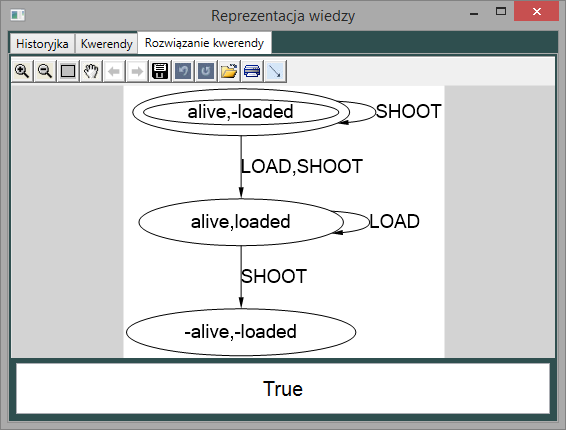
\includegraphics[scale=0.5]{test1_1}
    \end{figure}
    \item {\large\texttt{always accessible $\neg$alive}}\\
    Odpowiedź: \texttt{FALSE}\\
    Jest to prawda, ponieważ nie wszystkie ciągi akcji prowadzą do stanu, który spełnia podany warunek.
    \begin{figure}[H]
    \centering
    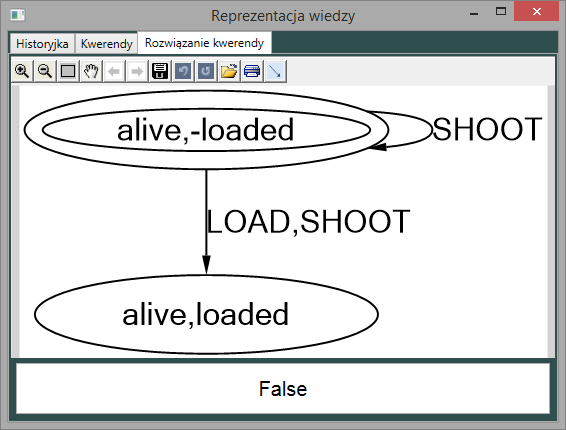
\includegraphics[scale=0.5]{test1_2}
    \end{figure}
    \item {\large\texttt{ever $\neg$alive after SHOOT, LOAD}}\\
    Odpowiedź: \texttt{FALSE}\\
    Jest to odpowiedź poprawna, ponieważ ze stanu początkowego, w którym zmienna $loaded$ nie jest prawdziwa, akcje $SHOOT$ i $LOAD$ nie zmienią stanu zmiennej $alive$.
    \begin{figure}[H]
    \centering
    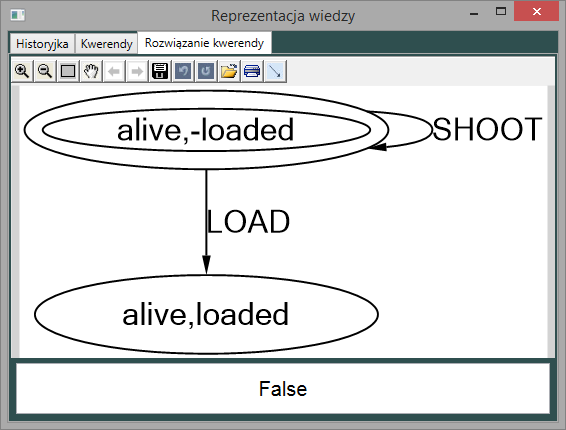
\includegraphics[scale=0.5]{test1_3}
    \end{figure}
    \item {\large\texttt{always executable SHOOT, LOAD, SHOOT}}\\
    Odpowiedź: \texttt{TRUE}\\
    Odpowiedź jest zgodna z prawdą - w dziedzinie nie istnieją zadania, które miałyby uniemożliwiać wykoanie ciągu podanych akcji.
    \begin{figure}[H]
    \centering
    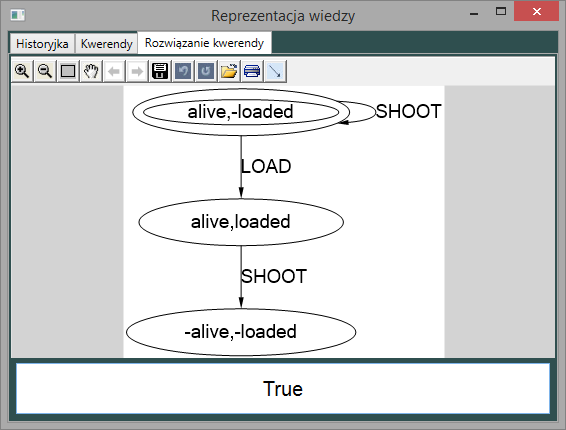
\includegraphics[scale=0.5]{test1_4}
    \end{figure}
\end{itemize}

\newpage
\subsection{Test 2}
Zdefiniowana dziedzina:
\bigskip
\lstset{
	style=main,
	keywords=[2]{Eat, Shop, Cook},
}
\begin{lstlisting}[mathescape=true]
initially hungry $\wedge$ angry
initially emptyFridge $\wedge$ $\neg$hasMeal $\wedge$ $\neg$chaos 
impossible Eat if $\neg$hasMeal 
impossible Cook if emptyFridge
Shop causes $\neg$emptyFridge
Shop releases angry if angry
Cook causes chaos if angry
Cook causes hasMeal 
Cook releases emptyFridge if emptyFridge
Eat causes $\neg$hasMeal $\wedge$ $\neg$hungry $\wedge$ $\neg$angry
\end{lstlisting}
\vspace{1cm}
Zadane kwerendy:
\begin{itemize}
    \item {\large\texttt{always executable COOK, SHOP}}\\
    Odpowiedź: \texttt{FALSE}\\
    Odpowiedż jest poprawna, ponieważ zdanie impossible uniemożliwia wykonanie akcji $COOK$ w przypadku gdy zmienna $emptyFridge$ jest prawdziwa.
    \begin{figure}[H]
    \centering
    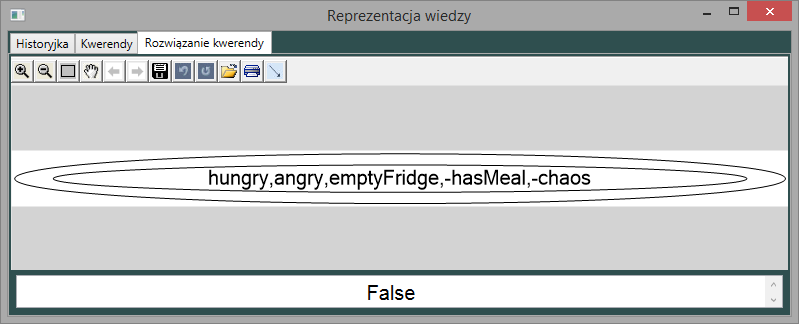
\includegraphics[scale=0.5]{test2_1}
    \end{figure}
    \item {\large\texttt{always executable \{COOK, SHOP\}}}\\
    Odpowiedź: \texttt{TRUE}\\
    Odpowiedż jest poprawna, ponieważ w tym wypadku zdefiniowana została akcja złożona z akcji $COOK$ i $SHOP$. Akcja $COOK$ nie jest wykonywalna ze stanu początkowego, więc pod uwagę brana jest tylko akcja $SHOP$, która jestw wykonywalna ze stanu początkowego. 
    \begin{figure}[H]
    \centering
    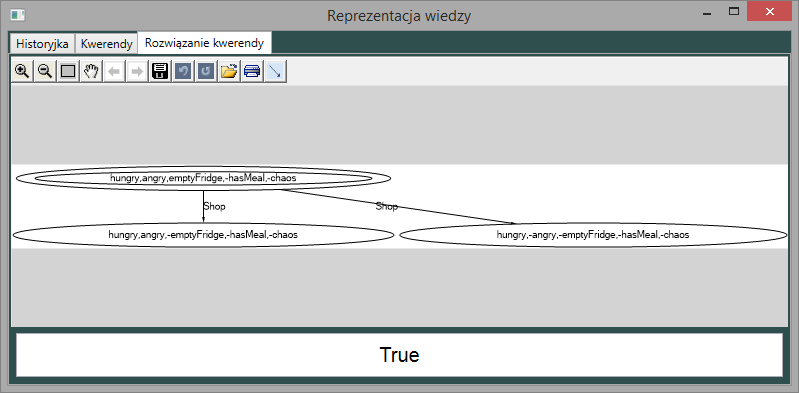
\includegraphics[scale=0.5]{test2_2}
    \end{figure}
    \item {\large\texttt{ever accessible emptyFridge $\wedge$ $\neg$angry $\wedge$ hungry $\wedge$ $\neg$chaos }}\\
    Odpowiedź: \texttt{TRUE}\\
    Jest to odpowiedź poprawna, jednak nie jest zrozumiałe, dlaczego w grafie zwróconym przez program widnieją stany, które nie spełniają podanych założeń i nie należą do ścieżki, która prowadzi do takiego stanu.
    \begin{figure}[H]
    \centering
    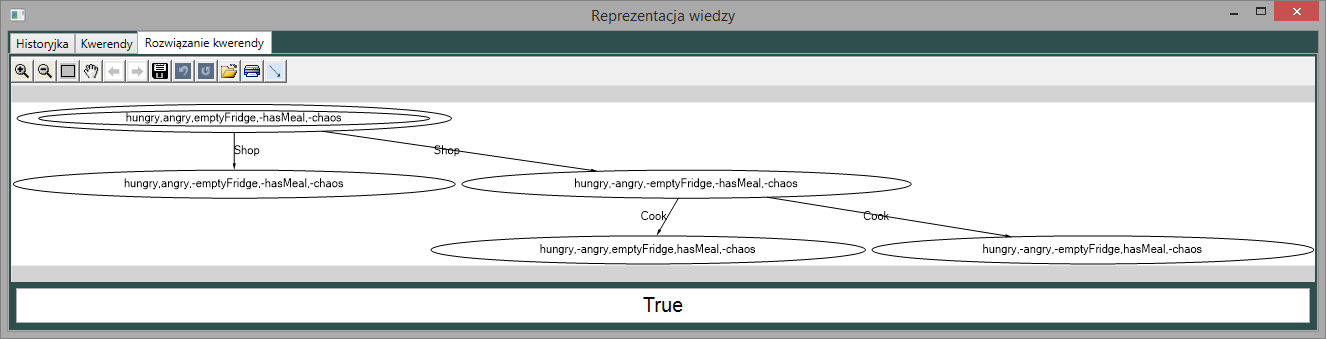
\includegraphics[scale=0.35]{test2_3}
    \end{figure}
    \item {\large\texttt{ever $\neg$emptyFridge after SHOP, COOK}}\\
    Odpowiedź: \texttt{TRUE}\\
    Odpowiedź jest zgodna z prawdą, ponieważ akcja $COOK$ może, ale nie musi zmienić stan zmiennej $emptyFridge$.
    \begin{figure}[H]
    \centering
    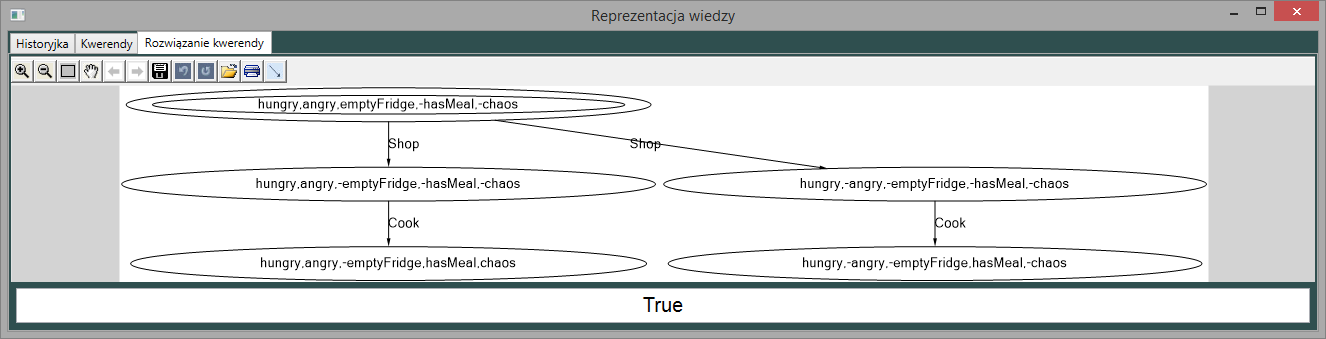
\includegraphics[scale=0.35]{test2_4}
    \end{figure}
\end{itemize}

\newpage
\subsection{Test 3 - kapelusznik w krainie czarów}
Zdefiniowana dziedzina:
\bigskip
\lstset{
	style=main,
	keywords=[2]{Eat, Drink},
}
\begin{lstlisting}[mathescape=true]
initially $\neg$hatterMad $\wedge$ cakeExists $\wedge$ elixirExists
drink causes hatterMad if elixirExists
eat causes $\neg$hatterMad
impossible eat if $\neg$cakeExists
drink releases elixirExists if elixirExists
eat causes $\neg$cakeExists
\end{lstlisting}
\vspace{1cm}
Zadane kwerendy:
\begin{itemize}
    \item {\large\texttt{ever cakeExists after eat}}\\
    Oczekiwana odpowiedź: \texttt{FALSE}\\
    Odpowiedź programu: \texttt{FALSE}\\
    Odpowiedż jest poprawna, ponieważ jedzenie zawsze powoduje brak ciastka, a w dziedzinie nie ma możliwości przywrócenia ciastka.
    \item {\large\texttt{always executable drink, drink}}\\
    Oczekiwana odpowiedź: \texttt{TRUE}\\
    Odpowiedź programu: \texttt{TRUE}\\
    Odpowiedż jest poprawna, ponieważ nawet jeśli eliksir się skończy, akcja picia jest wykonywalna.
    \item {\large\texttt{always accessible hatterMad}}\\
    Oczekiwana odpowiedź: \texttt{TRUE}\\
    Odpowiedź programu: \texttt{TRUE}\\
    Odpowiedź jest poprawna.
    \item {\large\texttt{ever ~hatterMad after drink, eat, drink, eat}}\\
    Oczekiwana odpowiedź: \texttt{FALSE}\\
    Odpowiedź programu: \texttt{FALSE}\\
    Odpowiedż jest poprawna - druga próba zjedzenia ciastka jest niewykonalna.
    \newpage
    \item {\large\texttt{ever $\neg$hatterMad after drink, eat, \{ drink, eat\} }}\\
    Oczekiwana odpowiedź: \texttt{TRUE}\\
    Odpowiedź programu: \texttt{TRUE}\\
    Odpowiedż jest poprawna, ścieżkę można zobaczyć na poniższym obrazku.
    \begin{figure}[H]
    \centering
    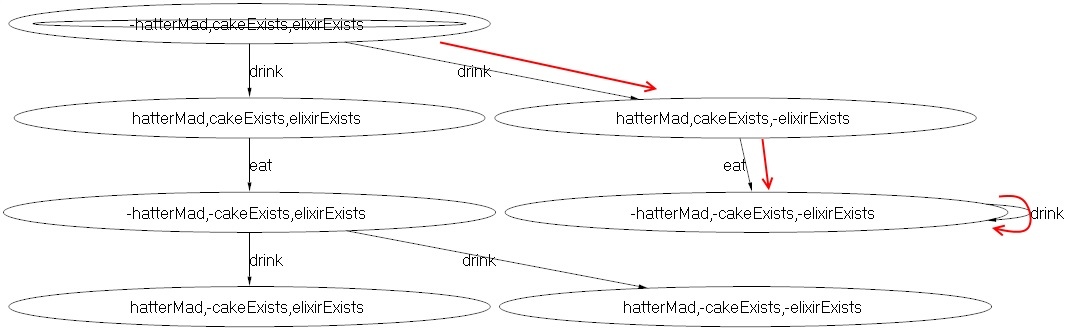
\includegraphics[scale=0.5]{test3_5}
    \end{figure}
    
    
    %\item {\large\texttt{?}}\\
    %Oczekiwana odpowiedź: \texttt{}\\
    %Odpowiedź programu: \texttt{}\\
    %Odpowiedż jest poprawna, ponieważ .
\end{itemize}

\newpage
\subsection{Test 4 - historia z indykiem i strzelającym Sebastianem}
Zdefiniowana dziedzina:
\bigskip
\lstset{
	style=main,
	keywords=[2]{Eat, Drink},
}
\begin{lstlisting}[mathescape=true]
initially loaded & $\neg$walking & alive
Shoot causes $\neg$loaded
Unload causes $\neg$loaded
Load causes loaded
Shoot causes $\neg$alive if $\neg$walking
Shoot releases alive if loaded & alive & walking
Shoot causes $\neg$walking if loaded
Entice causes walking
impossible Entice if $\neg$alive
\end{lstlisting}
\vspace{1cm}
Zadane kwerendy:
\begin{itemize}
	\item {\large\texttt{ever alive after Entice, Shoot, Load, Entice, Load, Shoot, Load, Shoot}}\\
	Oczekiwana odpowiedź: \texttt{FALSE}\\
	Odpowiedź programu: \texttt{FALSE}\\
	Odpowiedż jest poprawna, ponieważ indyk zaczyna chodzić po pierwszej akcji Entice co powoduje, że strzał może się nie udać. Jednak po strzale oddanym z nabitej broni indyk przestaje się ruszać (boi się). W takim wypadku strzał zawsze uśmierci biedne zwierzę.
	\begin{figure}[H]
		\centering
		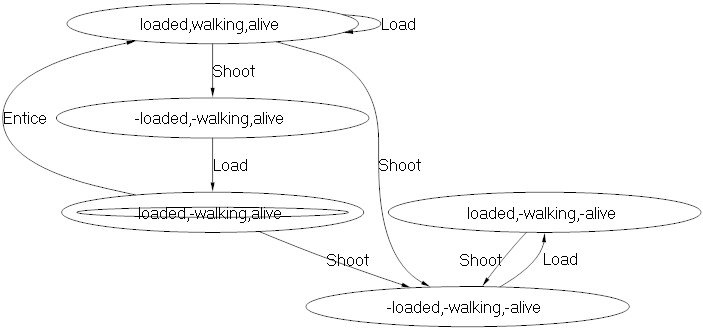
\includegraphics[scale=0.6]{kwerenda1}
	\end{figure}
	
	\item {\large\texttt{ever executable Load, Shoot, Entice}}\\
	Oczekiwana odpowiedź: \texttt{FALSE}\\
	Odpowiedź programu: \texttt{FALSE}\\
	Odpowiedż jest poprawna, ponieważ w przypadku naładowanej broni, kiedy indyk się nie porusza, strzał zawsze go uśmierci. Nie można wykonać akcji Entice w przypadku uśmierconego indyka.
	\begin{figure}[H]
		\centering
		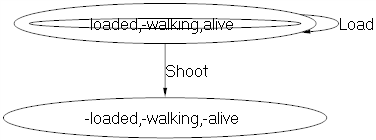
\includegraphics[scale=0.6]{kwerenda2}
	\end{figure}
	
	\item {\large\texttt{ever executable Unload, Shoot, Entice}}\\
	Oczekiwana odpowiedź: \texttt{TRUE}\\
	Odpowiedź programu: \texttt{TRUE}\\
	Odpowiedź jest poprawna. W przeciwieństwie do poprzedniej kwerendy, tutaj akcja Unload rozładowuje broń. Strzał z takiej broni nie uśmierci zwierzaka.
	\begin{figure}[H]
		\centering
		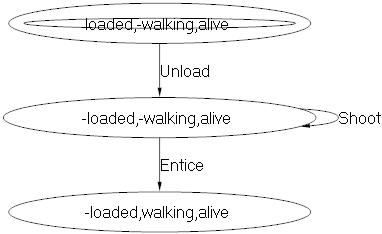
\includegraphics[scale=0.6]{kwerenda3}
	\end{figure}
	
	\item {\large\texttt{ever accessible ~alive}}\\
	Oczekiwana odpowiedź: \texttt{TRUE}\\
	Odpowiedź programu: \texttt{TRUE}\\
	Odpowiedż jest poprawna - indyka zawsze można w pewien sposób uśmiercić.
	\begin{figure}[H]
		\centering
		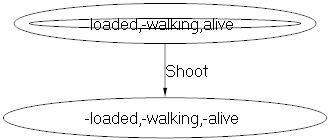
\includegraphics[scale=0.6]{kwerenda4}
	\end{figure}
	
	\item {\large\texttt{ever walking after Entice, Shoot, Load, Entice}}\\
	Oczekiwana odpowiedź: \texttt{TRUE}\\
	Odpowiedź programu: \texttt{TRUE}\\
	Odpowiedż jest poprawna - jeśli indyk się porusza strzał może się nie udać. Ponowne wykonanie akcji Entice spowoduje dalsze chodzenie zwierzaka.
	\begin{figure}[H]
		\centering
		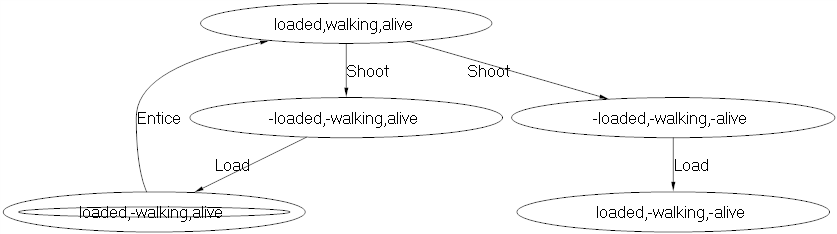
\includegraphics[scale=0.6]{kwerenda5}
	\end{figure}
\end{itemize}
\newpage
\subsection{Test 5 - Piwo i czipsy}
Stefan prowadzi mało zdrowy tryb życia: lubi jeść czipsy, pić piwo i oglądać telewizję. Z tego powodu ma mało pieniędzy. Do sklepu daleko, więc jak Stefan raz pojedzie na zakupy, to nie ma już pieniędzy na kolejny wypad do sklepu. Kiedy je czipsy, przestaje być głodny. Pragnienie może zaspokoić piwkiem, ale istnieje wtedy szansa, że znowu zgłodnieje. Stefan lubi również oglądać telewizję, ale robi to tylko wtedy, gdy nie jest ani głodny, ani spragniony. Szczęście Stefanowi zapewnia bezpośrednio tylko oglądanie telewizji. Obecnie Stefan jest i głodny, i spragniony, ma forsę ale nie jest szczęśliwy.Czy uśmiech ma szansę kiedykolwiek zagościć na jego twarzy?\\
Zdefiniowana dziedzina:
\bigskip
\lstset{
	style=main,
	keywords=[2]{Eat, Drink},
}
\begin{lstlisting}[mathescape=true]

drinkBeer causes $\neg$thirsty & $\neg$hasMoney if hasMoney
drinkBeer releases hungry if $\neg$hungry
eatChips causes $\neg$hungry & $\neg$hasMoney if hasMoney

watchTv causes happy if $\neg$hungry & $\neg$thirsty
impossible watchTv if hungry | thirsty

initially hungry & thirsty & $\neg$happy & hasMoney
\end{lstlisting}
\vspace{1cm}
Zadane kwerendy:
\begin{itemize}
	\item {\large\texttt{ever accessible happy}}\\
	Oczekiwana odpowiedź: \texttt{TRUE}\\
	Odpowiedź programu: \texttt{TRUE}\\
	Można dostać się do stanu $happy$, ale tylko, jeżeli wcześniej na raz wykona się akcje $drinkBeer$ i $eatChips$.
	\begin{figure}[H]
		\centering
		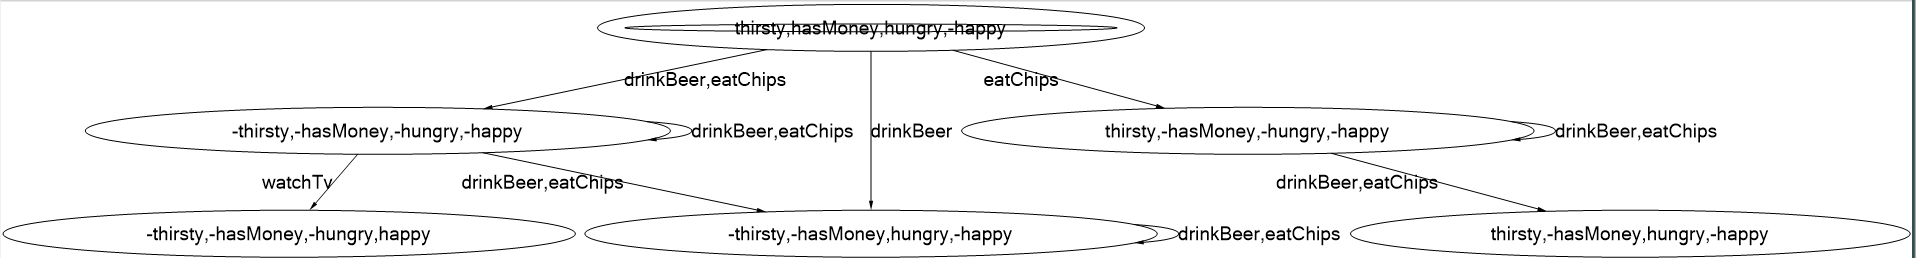
\includegraphics[scale=0.3]{stefan1}
	\end{figure}
\end{itemize}

\newpage
\subsection{Test 6}

\begin{center}
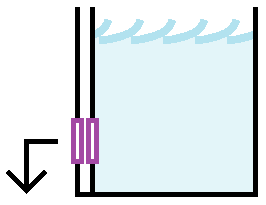
\includegraphics[scale=1]{test6_1}
\end{center}

Rozważmy zbiornik z wodą. Posiada on dwie szeregowo zainstalowane śluzy umożliwiające spuszczanie z niego zawartości. Śluzy można dowolnie otwierać i zamykać, przy czym zbiornik opróżnia się tylko wtedy, gdy obie śluzy są otwarte jednocześnie. Raz opróżnionego zbiornika nie można ponownie napełnić. Początkowo obie śluzy są zamknięte, a zbiornik wypełniony.

\bigskip
\noindent
Zdefiniowana dziedzina:
\lstset{
	style=main,
	keywords=[2]{OpenA, OpenB, CloseA, CloseB},
}
\begin{lstlisting}[mathescape=true]
initially $\neg openedA \wedge \neg openedB \wedge water $
OpenA causes $openedA$
OpenB causes $openedB$
OpenA causes $\neg water$ if $openedB$
OpenB causes $\neg water$ if $openedA$
\end{lstlisting}

\noindent
(dziedzina początkowo miała wykorzystywać zdanie \textbf{nonintertial}, jednak brak obsługi przez system zdania integralności \textbf{always} uniemożliwia jego praktyczne zastosowanie)

\bigskip
\noindent
Zadane kwerendy:

\begin{itemize}
    \item \textit{Czy sekwencyjne otwarcie śluz sprawia, że woda pozostaje w zbiorniku?}
    \medskip \\
    {\large\texttt{ever} $water$ \texttt{after} \normalsize \textsc{OpenA, OpenB}}\\
    Oczekiwana odpowiedź: \texttt{FALSE}\\
    Odpowiedź programu: \texttt{FALSE}
    
    \item \textit{Czy jednoczesne otwarcie śluz sprawia, że woda pozostaje w zbiorniku?}
    \medskip \\
    {\large\texttt{ever} $water$ \texttt{after} \normalsize \textsc{\{OpenA, OpenB\}}}\\
    Oczekiwana odpowiedź: \texttt{FALSE}\\
    Odpowiedź programu: \texttt{TRUE}    
    
    \item \textit{Czy jest możliwy stan, w którym śluzy są otwarte, a w zbiorniku pozostaje woda?}
    \medskip \\
    {\large\texttt{always accessible} $water \wedge openedA \wedge openedB$}\\
    Oczekiwana odpowiedź: \texttt{FALSE}\\
    Odpowiedź programu: \texttt{TRUE}
    
    
\end{itemize}

\newpage
\subsection{Test 7}
\newpage
\subsection{Test 8}
\newpage
\subsection{Test 9}
\newpage
\section{Wnioski}

\end{document}
